%%%%%%%%%%%%%%%%%%%%% chapter.tex %%%%%%%%%%%%%%%%%%%%%%%%%%%%%%%%%
%
% sample chapter
%
% Use this file as a template for your own input.
%
%%%%%%%%%%%%%%%%%%%%%%%% Springer-Verlag %%%%%%%%%%%%%%%%%%%%%%%%%%
%\motto{Use the template \emph{chapter.tex} to style the various elements of your chapter content.}
\chapter{Time Domain Numerical Methods}
\section{Finite Difference Time Domain Method}
The Finite Difference Time Domain (FDTD) Method is a numerical method for solving partial differential equations. The power of this method lies in simplicity and flexibility, and it can be used to solve partial differential equations of varying complexity~\cite{Schneider2015}. This chapter will discuss the application of the finite difference time domain method to the acoustic wave equation, including partially absorbing boundary conditions and the introduction of the sparse finite difference time domain method for acoustics.

\subsection{Introduction to the Finite Difference Time Domain Method}
Methods for solving partial differential equations have been of significant and continued research since the early 1900s. Mathematicians such as Courant, Fiedrichs and Hrennikof undertook seminal work in the early 1920s that formed a base for much of the finite methods used today. The FDTD Method is a numerical method for solving time domain problems (often wave equations) with localised handling of spatial derivatives, and was first introduced for solving Maxwell's equations to simulate electromagnetic wave propagation by Yee \cite{Yee1966}.\\

Yee proposed a method for solving Maxwell's equations in partial differential form by applying them to staggered matrices in partial steps of time and space. These matrices represented the magnetic (H) and electric (E) fields, where the relationship between H and E means one perturbs the other. In this explicit formulation H and E are solved contiguously in a 'leapfrog' style, executing two sets of computations to solve for one time step. Multiple time steps would be solved from current time $t = 0$, in steps of $dt$ to the end of simulation time $T$.\\

Each field is solved at half steps in time from the other, thus H for the current time step $t + \delta t$ is calculated using the H values one time step ago $t$, and the E values half a time step ago $t + \frac{\delta t}{2} $. These two fields are also solved using central finite differences in space, in a staggered grid format i.e. E at index $x$ at time $t + \delta t$ is calculated using E at index $x$ at time $t$, and the finite difference between the local discrete values of H at $x - \frac{\delta x}{2} $ and at $x + \frac{\delta x}{2} $ at time $t + \frac{\delta t}{2}$.\\

As such it is possible to apply a simple 'kernel' across many discrete points in a domain to simulate electromagnetic wave propagation.\\
In acoustics FDTD can be used to simulate a wide range of problems such as diffraction and diffusion, aeroacoustic, meteorological \& environmental and mixed medium, without having to perform multiple simulations for different frequencies or simulation characteristics \footnote{as would have to be required in frequency domain simulations such as some Finite Element and Boundary Element simulations}. 

\subsection{The Finite Difference Time Domain Method Applied To The Acoustic Wave Equation}
The FDTD method applied to solving the acoustic wave equation follows a similar form to that of solving Maxwells Equations with FDTD~\cite{Schneider2015}. Bottledoorens~\cite{Botteldooren1993} seminal work applied the FDTD method to the acoustic wave equations for both Cartesian and quasi-Cartesian grid systems. As previously described in the room acoustics section, the linear acoustic wave equation is based on Newton's second law of motion, the gas law and the conservation of mass. The equation has the following form for changes in the pressure and velocity respectively within a volume:\\
\begin{center}
$\frac{\delta^2 p}{\delta t^2} = \frac{1}{c^2} \frac{\delta^2 p}{\delta t^2}$\\
$\frac{\delta^2 u}{\delta t^2} = \frac{1}{c^2} \frac{\delta^2 u}{\delta t^2}$\\
\end{center}
As pressure $p$ and velocity $u$ have a reciprocal relationship in a similar way to H and E, it is possible to rearrange the acoustic wave equation to reflect this relationship for an FDTD computation.

\subsection{Field Calculation}
When treating the 1 dimensional linear acoustic wave equation with the FDTD method, it is possible to treat the $p$ and $u$ terms separately in time using the opposing terms for reciprocal calculation. As such, the $p$ and $u$ terms are reformulated as follows:\\
\begin{center}
$\frac{\delta^2 p}{\delta t^2} = p - \frac{\delta t}{\rho_0 \delta x} \frac{\delta^2 u}{\delta t^{2}}$\\
$\frac{\delta^2 u}{\delta t^2} = u - \frac{\delta t}{\rho_0 \delta x} \frac{\delta^2 p}{\delta t^{2}}$\\
\end{center}
This formulation is not in discrete time and space as is necessary when applying the FDTD method. As the FDTD method relies on solving local finite difference approximations across a domain of interest, it is important to define a space and time index referencing method. In many mathematical texts, time step indexing is often represented by an $i$ notation, and spatial indexing often uses the $j,k,l$ notation. For the sake of simplicity, in this study $t$ will denote the time step index, and $x$, $y$ and $z$ will denote spatial indexing in each dimension in a similar way to the standard world coordinates system of many computer aided design packages.\\
Following an implementation of the acoustic FDTD method by Hill~\cite{Hill2012}, the following discrete time and space $p$ and $u$ equations can be described:\\
\begin{center}
$u^{t + \frac{\delta t}{2}}_{x} = u^{t - \frac{\delta t}{2}}_{x} - \frac{\delta t}{\rho \delta x} \left[p^{t}_{x + \frac{\delta x}{2}} - p^{t}_{x - \frac{\delta x}{2}}\right]$\\
$p^{t + \frac{\delta t}{2}}_{x} = p^{t - \frac{\delta t}{2}}_{x} - \frac{c^2 \rho \delta t}{\delta x} \left[u^{t}_{x + \frac{\delta x}{2}} - u^{t}_{x - \frac{\delta x}{2}}\right]$\\
\end{center}
These update equations are developed for used with two matrices, one for for pressure values and one for velocity values. The size of these matrices is determined by the size of the domain of interest and the spatial step size. The spatial step size is determined by the highest frequency of interest and the number of grid points required per wavelength, which is often regarded as being between 6 and 10 points in much FDTD literature. The spatial step size has a significant impact on both simulation stability and execution time, and is discussed further in the report.
\newpage
\subsection{Block Diagram}
A basic block diagram of a program for solving the the acoustic FDTD method is given bellow:\\

% Define block styles
\tikzstyle{decision} = [diamond, draw, fill=blue!20, 
    text width=4.5em, text badly centered, node distance=3cm, inner sep=0pt]
\tikzstyle{block} = [rectangle, draw, fill=blue!20, 
    text width=5em, text centered, rounded corners, minimum height=4em]
\tikzstyle{line} = [draw, -latex']
\tikzstyle{cloud} = [draw, ellipse,fill=red!20, node distance=3cm,
    minimum height=2em]
    
\begin{tikzpicture}[node distance = 1.5cm, auto]
    % Place nodes
    \node [block] (init) {initialize model};
   %\node [cloud, left of=init] (expert) {expert};
   %\node [cloud, right of=init] (system) {system};
    \node [block, below of=init] (evaluateu) {update velocities};
    \node [block, below of=evaluateu] (evaluateb) {update boundaries};
    \node [block, below of=evaluateb] (evaluatep) {update pressures};
    \node [block, below of=evaluatep] (source) {add source terms};
    \node [block, below of=source] (record) {record at reciever, $t = t + \delta t$};
    \node [block, left of=evaluateb, node distance=3cm] (display) {display model};
    \node [decision, below of=record] (decide) {$t = T?$};
    \node [block, below of=decide, node distance=2cm] (stop) {stop and postprocess};
    % Draw edges
    \path [line] (init) -- (evaluateu);
    \path [line] (evaluateu) -- (evaluateb);
    \path [line] (evaluateb) -- (evaluatep);
    \path [line] (evaluatep) -- (source);
    \path [line] (source) -- (record);
    \path [line] (record) -- (decide);
    \path [line] (decide) -| node [near start] {no} (display);
    \path [line] (display) |- (evaluateu);
    \path [line] (decide) -- node {yes}(stop);
    %\path [line,dashed] (expert) -- (init);
    %\path [line,dashed] (system) -- (init);
    %\path [line,dashed] (system) |- (evaluate);
\end{tikzpicture}

\subsection{Boundary Handling}
As a significant part of room acoustic simulation involves analysing the effects of reverberation, so it may be important to model a boundary (wall, ceiling, floor) that will absorb and reflect some proportion of energy that is at the boundary. This can be handled by calculating partial derivatives at the boundaries of the domain based on the acoustic impedance of the boundaries~\cite{Olesen1997}\cite{Hill2012} i.e. boundaries are handled at velocity points where one pressure point is available for the differentiation. $p$, $u$ and impedance $z$ are often applied in a relationship similar to Ohms law $v = i * r $. The absorbing and reflecting properties of boundaries in acoustics are often defined as normalised quantities related to the loss in energy when a portion of the material is tested under conditions such as energy loss time when placed in a reverberation chamber~\cite{Beranek2006}. The equation to calculate acoustic impedance based on absorption coefficient is as follows:\\
\begin{center}
$z = \rho c \frac{1 + \sqrt{1 - a}}{1 - \sqrt{1 - a}} $\\
\end{center}
Due to the spatially staggered grids in FDTD, it is possible to handle the outer boundaries of a rectilinear domain in the velocity components by increasing the size of the velocity matrices by 1 in the direction of the velocity i.e. the length of a 3 dimensional $u_x$ matrix would be:\\
\begin{center}
$u_{x_{x,y,z}} = (x = N+1, y = N, z = N)$ 
\end{center} Where the size of the $p$ matrix is:\\
\begin{center}
 $p_{x,y,z} = N:N:N$. 
\end{center}
For convenience and simplicity, local constant terms for the boundary can  be lumped into an R parameter:\\
\begin{center}
$R = \frac{\rho \delta x}{0.5 \delta t}$\\
\end{center} 
This parameter reflects the handling of the boundary differential only being a half-step in time. Rearranging the form of the velocity equation to include a the partial derivative acoustic impedance component at the negative x boundary can be given as follows:\\
\begin{center}
$ u^{t + \frac{\delta t}{2}}_{x} = \frac{R - Z}{R + Z} u^{t - \frac{\delta t}{2}}_{x} - \frac{2}{R + Z} p^{t}_{x+ \frac{\delta x}{2}} $\\
\end{center}
In this implementation of the FDTD method no internal obstacles are handled. In the study by Angus \textit{et al}~\cite{Angus2010}, obstacles were handled simply by setting local velocity  values to 0 imposing a totally hard boundary within the domain. An improvement to this may be to implement the absorbing boundary conditions discussed above to the outside velocity points of an obstacle, allowing the obstacles to partially absorb.

\subsection{Example Function for Solving}
Below, is a function written in the Matlab \textregistered language, used to solve one time step of the wave equation using the FDTD method, in 3 dimensions:
\lstinputlisting[language=Matlab]{../Matlab/FDTD/FDTD3Dfun.m}

\subsection{Stability}
Surrounding this formulation of the FDTD method for the acoustic wave equation, it may be important to ensure appropriate conditions are met for a converging and stable solution. As this is an explicit time marching method, the Courant-Friedrichs-Lewy (CFL) stability condition may provide a guide for generating appropriate spatial and temporal discretisation steps~\cite{Sakuma2014,Schneider2015,Angus2010,Bilbao2009,Hill2012}. The CFL condition implies that spatial $\delta x$ and temporal $\delta t$ discretization of a wave propagation model must be sufficiently small, that a single step in time is equal to or smaller than the time required for a wave to cross a spatial discretization step. This concerns both the speed of wave propagation $c$, the number of dimensions $N_D$ and maximum simulation frequency $f_{max}$. The 2 dimensional CFL condition can be computed as such, where the CFL limit $C_{max}$ is approximately 1 due to the use of an explicit time stepping solver:\\
\begin{center}
$ CFL = c \frac{\delta t}{\sqrt{\Sigma_{1}^{N_D} \delta {N_{D}}^2}} \leq C_{max}$\\
\end{center}
As the number of dimensions increases and the spatial step decreases, the time step must decrease for the simulation to remain stable. Although a simulation must have a CFL coefficient that is less than the $C_{max}$, this does not guarantee numerical stability and there is a lower limit of time step that can be observed in a poorly defined simulation.\\
As this acoustic simulation is a discrete computation of a continuous system, the Nyquist sampling theorem must be considered. This suggests that $\delta t \leq \frac{f_{max}}{2}$. It has been suggested in various studies~\cite{Hill2012,VanMourik2014} that between 5 and 10 points per shortest wavelength are required for accurate stable simulation $\delta_x = c / (\textit{f}_{max} 6)$. As $\delta x$ and $\delta t$ are linked by the CFL condition, $\delta t \leq \frac{\frac{1}{c} \delta_x}{2}$. Stability analysis techniques are available for analysing the stability of simply shaped unbounded models such as VonNeuman analysis~\cite{Bilbao2009,Hamilton2013a}. Due to time constraints VonNeuman Analysis was not implemented in this study.

\section{Sparse FDTD}
\subsection{Introduction to the Sparse Finite Difference Time Domain Method}
The sparse FDTD method (SFDTD) is a variant of the FDTD method proposed by Doerr~\cite{Doerr2013} for use in the modelling of optical problems with significantly large domains such as PIC micro-controllers. This is not to be confused with sparse matrix solvers used for decomposing large sparse matrices in implicit FDTD methods. The SFDTD method relies on setting an appropriate threshold, and uses this threshold to determine points in the simulation domain that should be solved and points that should be ignored. This is analogous to applying a gate or window to the domain being computed, where ignoring parts of the domain with sufficient energy may significantly reduce computation time.\\

The approach suggested by Doerr is similar to the moving window FDTD method implemented by Schuster \textit{et al}~\cite{Schuster2004}, in that the number of computations undertaken at any one time is significantly reduced and may improve computation time in a large simulation. However unlike moving window FDTD, the SFDTD implementation suggested by Doerr dynamically accommodates high and low energy points as the simulation continues. This is achieved by maintaining a set of lists of currently active points, previously active points and a matrix that parallels the domain and contains list indices. Doerr's method relies on constantly maintaining lists, and a pointing array that is the same size as the domain.\\

Maintaining multiple large lists in memory may be detrimental to the speed of execution in of a large system where non-contiguous memory accesses are expensive in time. This may be of further concern when considering the difference in behaviour between electromagnetic and acoustics waves. Electromagnetic waves are transverse and can travel through a vacuum, acoustic waves are longitudinal and mechanical i.e. are fluctuations in a medium. Mechanical waves diffuse but photons in a PIC simulation may not, and the addressing of multiple lists with diffusing mechanical waves may be less practical than in PIC simulations. As such another method of windowing is explored below. \\

\subsection{Acoustic Implementation of SFDTD in Two Dimensions}
The implementation of the SFDTD for 2D simulation in this study attempts to leverage some signal processing techniques instead of search algorithms or individual checks like Doerrs method. The aim of is to generate a single indexing matrix as opposed to having an indexing matrix and lists. The points of the matrix will be used as a mask, where points with an absolute pressure above a threshold and surrounding points will be computed.\\

The domains of interest in this study are large and contain many points. To generate index points around those with adequate pressure to be calculated, some smoothing of the pressures in the matrix is required. This could be thought of as similar to a blurring effect or smoothing in image processing~\cite{Blanchet2006}, which is the process of convolving an image with a Gaussian function and essentially low-pass filtering the image. This process reduces noise and details of an image, and thus should smooth around the threshold window and allow the processing mask in the SFDTD method to work just outside of the confines of the areas where the pressure is above the threshold. Below is a Matlab function for calculating such a matrix:\\

\lstinputlisting[language=Matlab]{../Matlab/SFDTD/SPARSEfun2DC.m}

Below is an example surf plot of the indexing matrix for a 50m by 40m simulation with a maximum sampling frequency of $1kHz$ and a windows threshold of 40dB. 
\begin{figure}[H]
\centering
  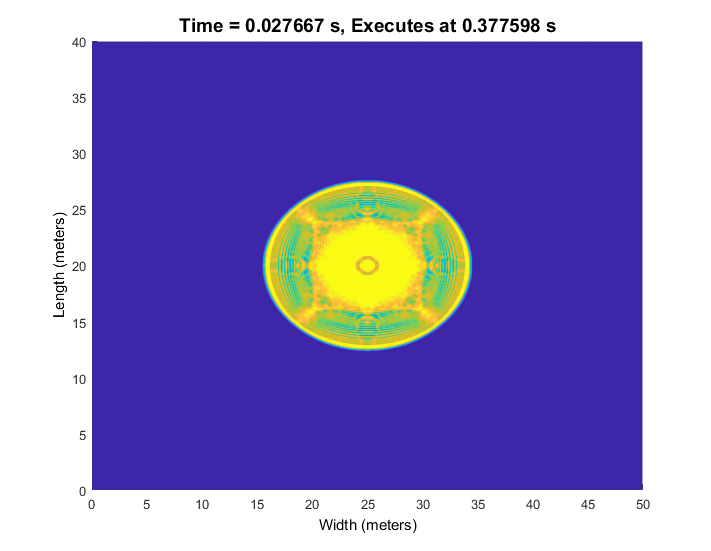
\includegraphics[width=0.75\textwidth]{./graphics/Example Window 1.png} %./graphics/Example Window 1.png
  \caption{Window of an expanding wave in an SFDTD simulation}
\end{figure}
It can be seen that the dispersion error caused by the rectilinear system is imprinted on the window. Dispersion error is the phase error with which different frequencies travel in an FDTD simuation~\cite{Saarelma2016}, and low order staggered schemes may sufferd consideribly from this error. There is ongoing research as to the perceptual effects of disperison error in different FDTD schemes, when calculating impulse responses for auralization. Further experimentation using a higher order FDTD scheme may reduce numerical dispersion~\cite{Hamilton2013a,VanMourik2014} and improve the effectiveness of the window in reducing computation area to wave-fronts.\\

The figure below shows the window shape for a similar simulation to the one above, but with a threshold of 60dB.\\
\begin{figure}[H]
\centering
  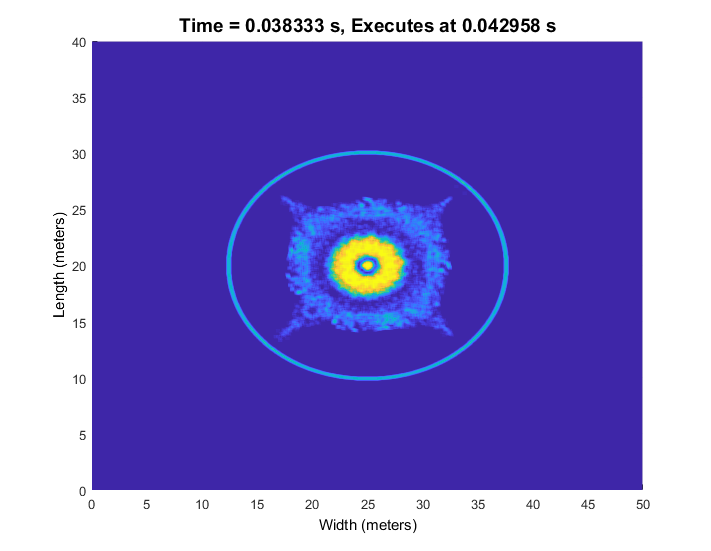
\includegraphics[width=0.75\textwidth]{./graphics/Example Window 3 60 threshold.png}
  \caption{Window of an expanding wave in an SFDTD simulation}
\end{figure}

It can be seen that the dispersion trailing the outer wave-front has been truncated. This is reflected in the figure below that shows the power spectrum for a receiver 12m away from the sound source for three simulations. This suggests that the SFDTD methods is essentially reducing the level of the spectrum, and is reducing the signal to noise ratio. Below is a plot of the execution speed of time steps as the same simulations progress, for a number of threshold: \\

\begin{figure}[H]
\centering
  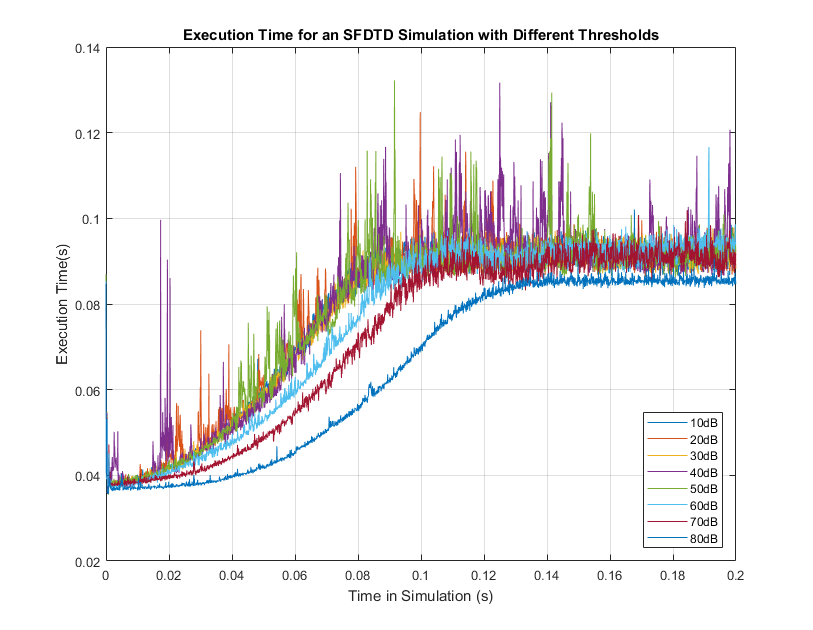
\includegraphics[width=\textwidth]{./graphics/sfdtd execution speed.png}
  \caption{Smoothed rate of time step execution for the SFDTD method during simulations, for different threshold levels}
\end{figure}

The figure below shows that simulations in small domains using the SFDTD method can still exhibit tradition wave patterns:\\

\begin{figure}[H]
\centering
  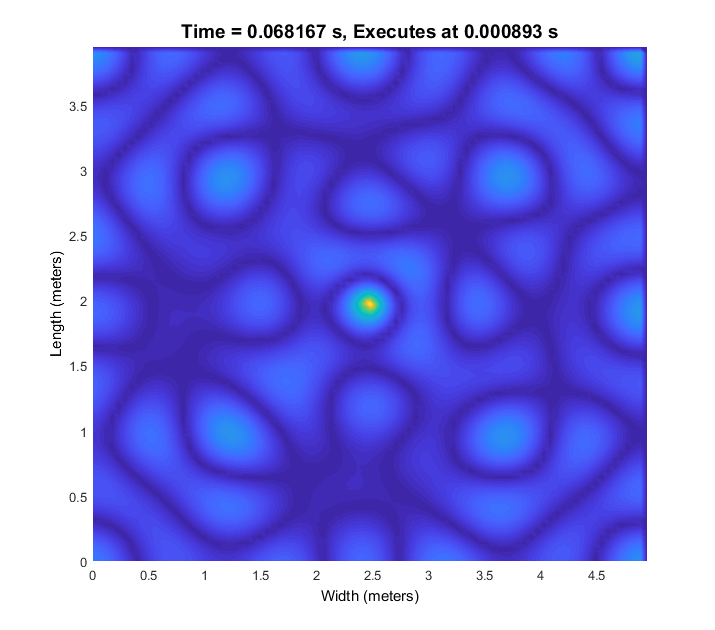
\includegraphics[width=0.75\textwidth]{./graphics/sfdtd with wave shapes.png}
  \caption{Single source SFDTD simulation in a small room with nodes and anti-nodes present}
\end{figure}

It can be seen that increasing the threshold level of the windowing function decreases arrogate and individual execution times, and begins to become much faster with a threshold above 40dB.
The FDTD algorithm above is adjusted to reference this matrix and operate at non-zero coordinates, calculating not only the regions with appropriate amounts of power but also the surrounding cells. The current implementation uses an if statement which is potentially very slow, and would not be easy to solve in parallel arithmetically. As well as implementing this method in 3D, it may be crucial to develop a method for masking the simulation and solving without using any if statements. Depending on the simulation, the level of the threshold value may be set as a single value or may be set to decrease over time to accommodate diffuse field calculation. However if an appropriate lossy wave equation was implemented, it may be possible to use a relatively high threshold to compute propagation loss for wave-fronts such as strong and early reflections.\\












